\subsection{Methane pyrolysis in shock-tube}

The pyrolysis of a 5\% $\mathrm{CH_4}$–Ar mixture was studied using the CPR model over a post-shock temperature range of $\mathrm{T_5} = 1800$–$3000$ K and a pressure range of $\mathrm{P_5} = 4.7$–$7.1$ bar. Since $\mathrm{P_5}$ was not specified for individual experiments (each defined by a given $\mathrm{T_5}$), a linear dependence of $\mathrm{P_5}$ on $\mathrm{T_5}$ was assumed within the stated range~\citep{agafonov2016unified}. Gas-phase chemistry was modeled using the Caltech mechanism. Inception and PAH adsorption rates were adjusted using $\eta_{inc}$ and $\eta_{ads}$, respectively, to match the predicted Carbon Yield (CY) at $t = 1.5$ ms with light extinction measurements at $\lambda = 632$ nm across the studied $\mathrm{T_5}$ and $\mathrm{P_5}$ ranges~\citep{agafonov2016unified}. The experimental CY was extracted from the reported product CY$\times$E(m). However, this approach introduces uncertainty due to variability in E(m). It is common to assume the E(m) of mature soot, which may not be valid in shock tube experiments with short residence times ($\approx 2$ ms) that involve initial stages of soot formation, as E(m) increases with particle size, composition, and maturity. For instance, during acetylene pyrolysis, E(m) can vary from 0.05 to 0.25 as the primary particle diameter reaches 20 nm within 1.6 ms. Despite such observations, our quantitative understanding of the evolution of E(m) in soot remains limited. We considered the reported variability of E(m) in the literature, ranging from 0.174~\citep{lee1981optical} to 0.37~\citep{agafonov2011soot}.

A parametric study was conducted on $\eta_{inc}$ and $\eta_{ads}$ using a grid search approach. Each factor was varied across 11 logarithmically spaced values from $10^{-4}$ to 1, resulting in 121 simulation cases per data point and 847 simulations in total. Each $\eta_{inc}$ and $\eta_{ads}$ pair was ranked based on the average relative error of CY across all data points in the studied $\mathrm{T_5}$ range, in order to identify the set of adjustment factors that minimized the CY prediction error. 

To reduce the computational load of the parametric study, simulations were performed using MPBM for all inception models. The comparison of results obtained using SPBM and MPBM shows that CY and $d_p$ are not sensitive to the choice of particle dynamics model, indicating that MPBM results can be reliably used for CY error analysis. However, $N_{agg}$ and $n_p$, shown in Figure~\ref{fig:shockagof_N_agg_n_p_cpr_pdynamics}, differ significantly between SPBM and MPBM because the central assumption of the monodisperse model is the rapid attainment of SPSD, which is not valid at short residence times near 1.5~ms. For example, the non-dimensional PSD at $\mathrm{T_5}=2200$~K, shown in Figure~\ref{fig:shockagof_psd}, significantly changes from 1.0~ms to 2.5~ms for all inception models.

Figure~\ref{fig:shockagof_yielderror_cpr} shows a heat map of the mean relative error, normalized by the maximum value, for all inception models. The largest error occurs for the combination of maximum inception ($\eta_{inc} = 1$ or $\log_{10}(\eta_{inc}) = 0$) and minimum adsorption ($\eta_{ads} = 10^{-4}$ or $\log_{10}(\eta_{ads}) = -4$). The region of lowest normalized error (less than 5\%), outlined in blue in Figure~\ref{fig:shockagof_yielderror_cpr}, includes a broad set of adjustment factor combinations that enable the model to accurately predict CY. However, accurate prediction of CY does not necessarily imply accurate prediction of other properties, such as primary particle diameter or mobility diameter. The availability of data on other soot parameters or intermediate gaseous species, and including them as optimization targets, could help narrow down the range of optimal adjustment factors.

To highlight the variability in soot morphology across the low-error region of the heat map, we focus on three representative combinations of $\eta_{inc}$ and $\eta_{ads}$: (i) minimum inception flux ($\eta_{inc} = 10^{-4}$), (ii) minimum PAH adsorption rate ($\eta_{ads} = 10^{-4}$), and (iii) equally scaled inception flux and PAH adsorption rate ($\eta_{inc} \approx \eta_{ads}$). It is important to note that soot CY and morphology are closely coupled to gas-phase chemistry under the short residence times studied. Therefore, a set of simulations was performed without soot to isolate gas-phase chemistry and examine the temperature dependence of soot precursors and $\mathrm{C_2H_2}$. Subsequently, inception models were optimized using equal adjustment factors ($\eta_{inc} = \eta_{ads}$), and separate optimizations were carried out for the minimum adsorption case ($\eta_{ads} = 10^{-4}$) and the minimum inception case ($\eta_{inc} = 10^{-4}$), denoted as \textit{Min-Ads} and \textit{Min-Inc}, respectively.


\begin{figure}[H]
	\centering
	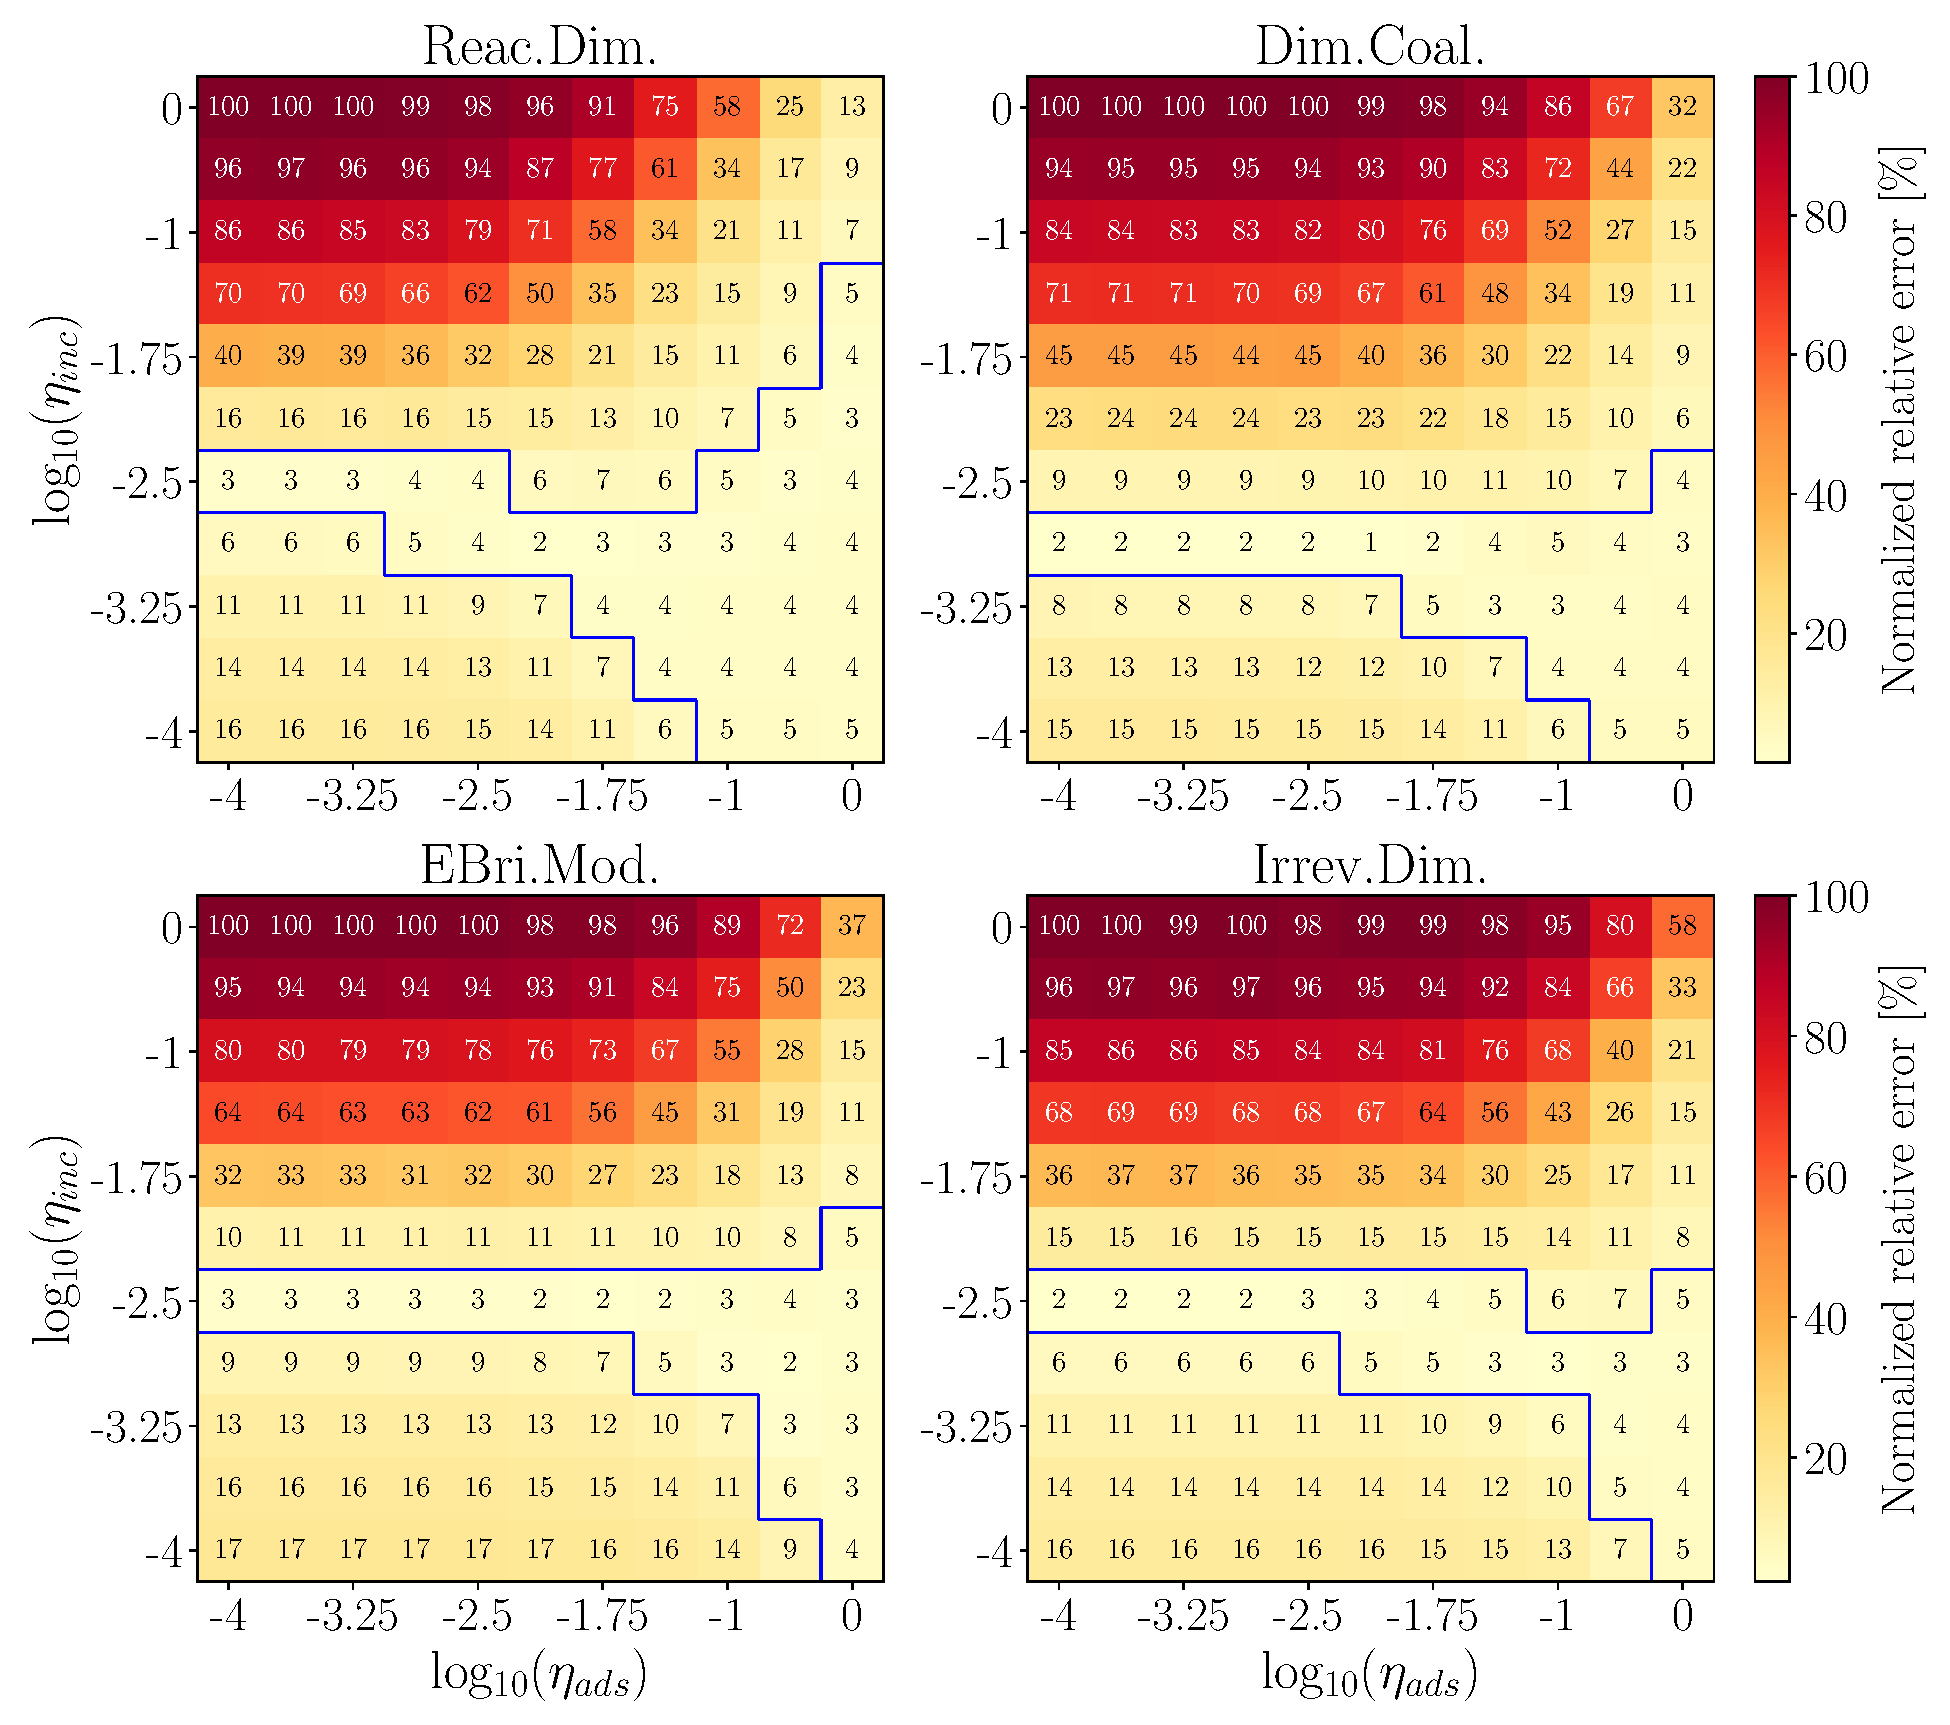
\includegraphics[width=0.8\textwidth]{Figures/Results/Shocktube/Agafonov2016_cpr/5CH4_norm_yield_error_all.pdf}
	\caption{The relative error of CY normalized by the maximum value at $t=1.5$ ms for 5\%~$\mathrm{CH_4}$-Ar obtained using Caltech mechanism and different inception models.}
	\label{fig:shockagof_yielderror_cpr} 
\end{figure}

Figure~\ref{fig:SPC_cmf_cpr}a shows the CMF of soot precursors (individual PAHs and total) and $\mathrm{C_2H_2}$ at 1.5 ms across the studied temperature range, with the soot model deactivated. While PAH precursors exhibit a bell-shaped profile, the CMF of $\mathrm{C_2H_2}$ increases linearly with temperature and plateaus near 85\% at $\mathrm{T_5} \approx 2400$ K. Among the considered PAHs, A2, A2R5, and A4R5 account for most of the carbon and are likely major contributors to soot inception and surface growth. The strong variation in PAH CMF highlights the impact of precursor selection on inception flux, surface growth rates, and their temperature dependence. Figure~\ref{fig:shockagof_yieldspc_cpr} illustrates the effect of excluding five-membered ring PAHs (A2R5, A3R5, and A4R5) from the soot precursors on the CY and $d_p$. As expected, excluding these species reduces CY for all inception models potentially highlighting the significant contribution of five-membered rings PAHs. The majority of carbon mass of PAHs in soot particles over 2000 K$<\mathrm{T_5}<$2400 K originates from A2R5 and A4R5 (Figure~\ref{fig:shockagof_spccont_cpr}).

\begin{figure}[H]
	\centering
	\begin{subfigure}[t]{0.4\textwidth}
		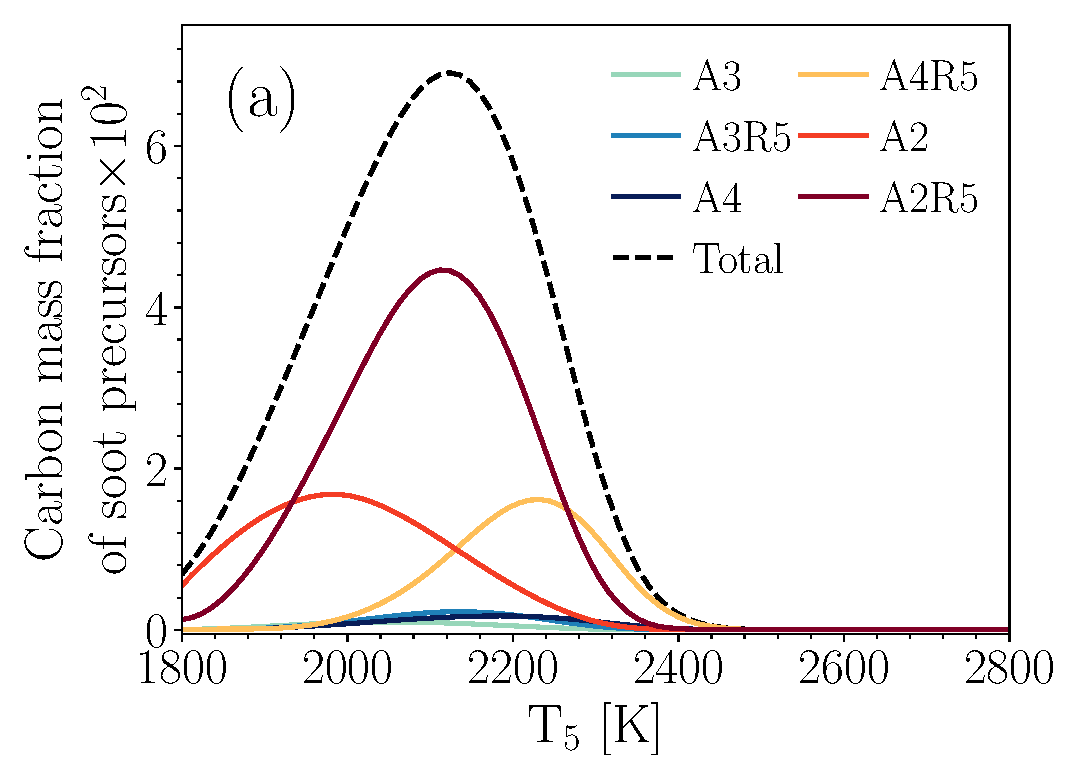
\includegraphics[width=1\textwidth]{Figures/Results/Shocktube/Agafonov2016_cpr/SPC_cmf_separate.pdf}
	\end{subfigure}
	\begin{subfigure}[t]{0.36\textwidth}
		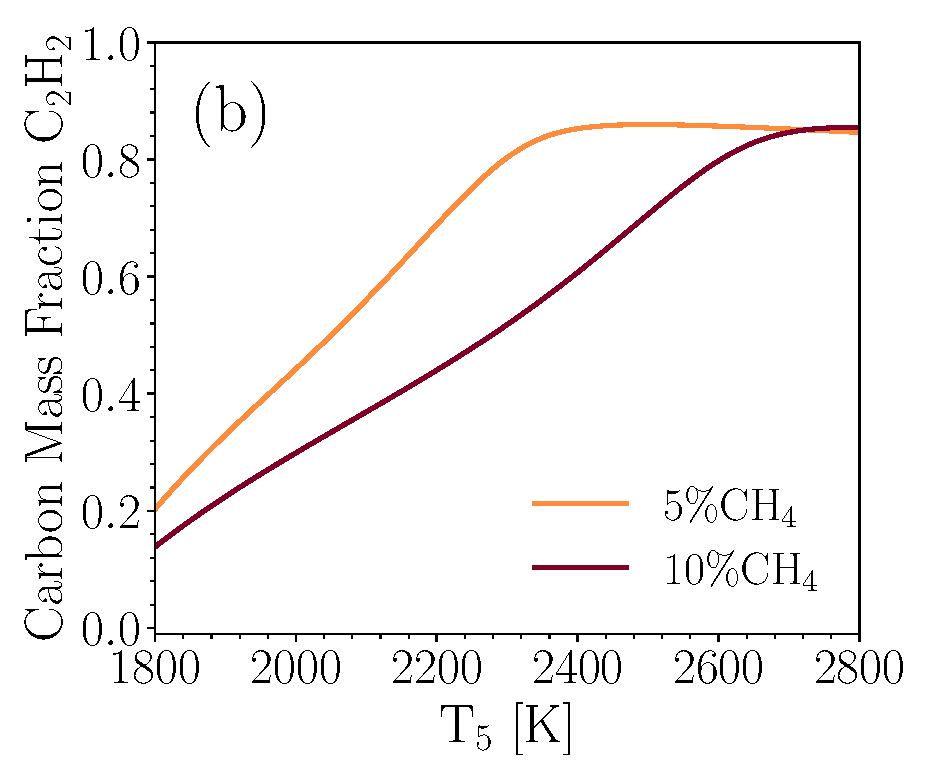
\includegraphics[width=1\textwidth]{Figures/Results/Shocktube/Agafonov2016_cpr/C2H2_cmf.pdf}
	\end{subfigure}
	\caption{The bell-shaped temperature profile of carbon mass fraction of soot precursors (A2 and larger) combined (a) and $\mathrm{C_2H_2}$ (b) at $t=$1.5 ms during pyrolysis of 5\% $\mathrm{CH_4}$-Ar (green line) obtained using CPR model with Caltech mechanism without considering soot.}
	\label{fig:SPC_cmf_cpr} 
\end{figure}





Next set of simulations were conducted by using equal adjustment factors ($\eta_{inc}=\eta_{ads}$) to minimize the prediction error of CY. Figure~\ref{fig:shockagof_yield_dp_cpr}a compares CY from various inception models with experimental data~\citep{agafonov2016unified}. A skew exponential curve (black dotted line) was fitted to the data to highlight the CY trend and its peak near 12\%. Soot CY follows a bell-shaped profile similar to that of soot precursors, as inception flux and mass growth directly depend on precursor concentrations. Reactive Dimerization model predicts higher CY at lower temperatures, while E-Bridge Modified model shifts the peak to higher temperatures due to a different temperature dependence, which is primarily governed by PAH dehydrogenation via an Arrhenius rate law, in contrast to physical PAH collisions in other models. 


As shown in Figure~\ref{fig:shockagof_yield_dp_cpr}b, the predicted $d_p$ increases with $\mathrm{T_5}$, reaching a maximum of 12.5 nm at 2700 K, where yield is very low ($\approx 10^{-7}$), and then drops to the model's minimum allowed value of 2 nm. The differences between inception models in predicting $d_p$ is overall negligible except for Reactive Dimerization model, which predicts a larger $d_p$ in $\mathrm{T_5}<2500$ K. The $d_p$ trends can be better understood by examining Equation~\eqref{eqn:d_p} indicating that $d_p$ is proportional to the third-root of $C_{tot}/N_{pri}$. $C_{tot}$ describes total carbon mass converted to soot through inception and surface growth while $N_{pri}$ is only determined by inception flux. As a result, $d_p$ is controlled by the ratio of total surface growth rate (via HACA and PAH adsorption) to inception flux. The ratio of carbon mass gained up to 1.5 ms by each pathway to the total soot carbon mass was calculated and shown in Figure~\ref{fig:shockagof_carbon_map_cpr}. PAH adsorption is the dominant soot mass growth pathway for Reactive Dimerization model in $\mathrm{T_5}<2000$ K (Figure~\ref{fig:shockagof_carbon_map_cpr}a), which results in larger $C_{tot}/N_{pri}$ and $d_p$ values, but inception is dominant for the other inception models. The contribution of inception decreases with temperature for all inception models while the contribution of HACA becomes dominant up to 2700 K leading to higher $d_p$ (Figure~\ref{fig:shockagof_yield_dp_cpr}b). This is due to the decrease of precursor concentration and the increase of $\mathrm{C_2H_2}$ CMF. Beyond 2700 K, the contribution of inception rapidly increases with temperature because leading to decrease of $d_p$ (Figure~\ref{fig:shockagof_yield_dp_cpr}b).


Figure~\ref{fig:shockagof_Nagg_np_cpr}a shows that $N_{pri}$ peaks near 2200 K, aligning with the peak in CY. This is expected because $N_{pri}$ depends solely on the inception flux, which is the highest when PAH concentrations peak. Increased coagulation rates reduce $N_{agg}$ in the $2000-2500$ K range. Reactive Dimerization model yields the fewest particles ($N_{pri}$ and $N_{agg}$) because more precursors are directed toward surface growth. Consequently, $n_p$ is lowest for Reactive Dimerization model. Differences between inception models are more evident in $n_p$ than in $d_p$, influencing predicted particle morphology.

\begin{figure}[H]
	\centering
	\begin{tikzpicture}
		\draw (0, 0) node[inner sep=0] 	{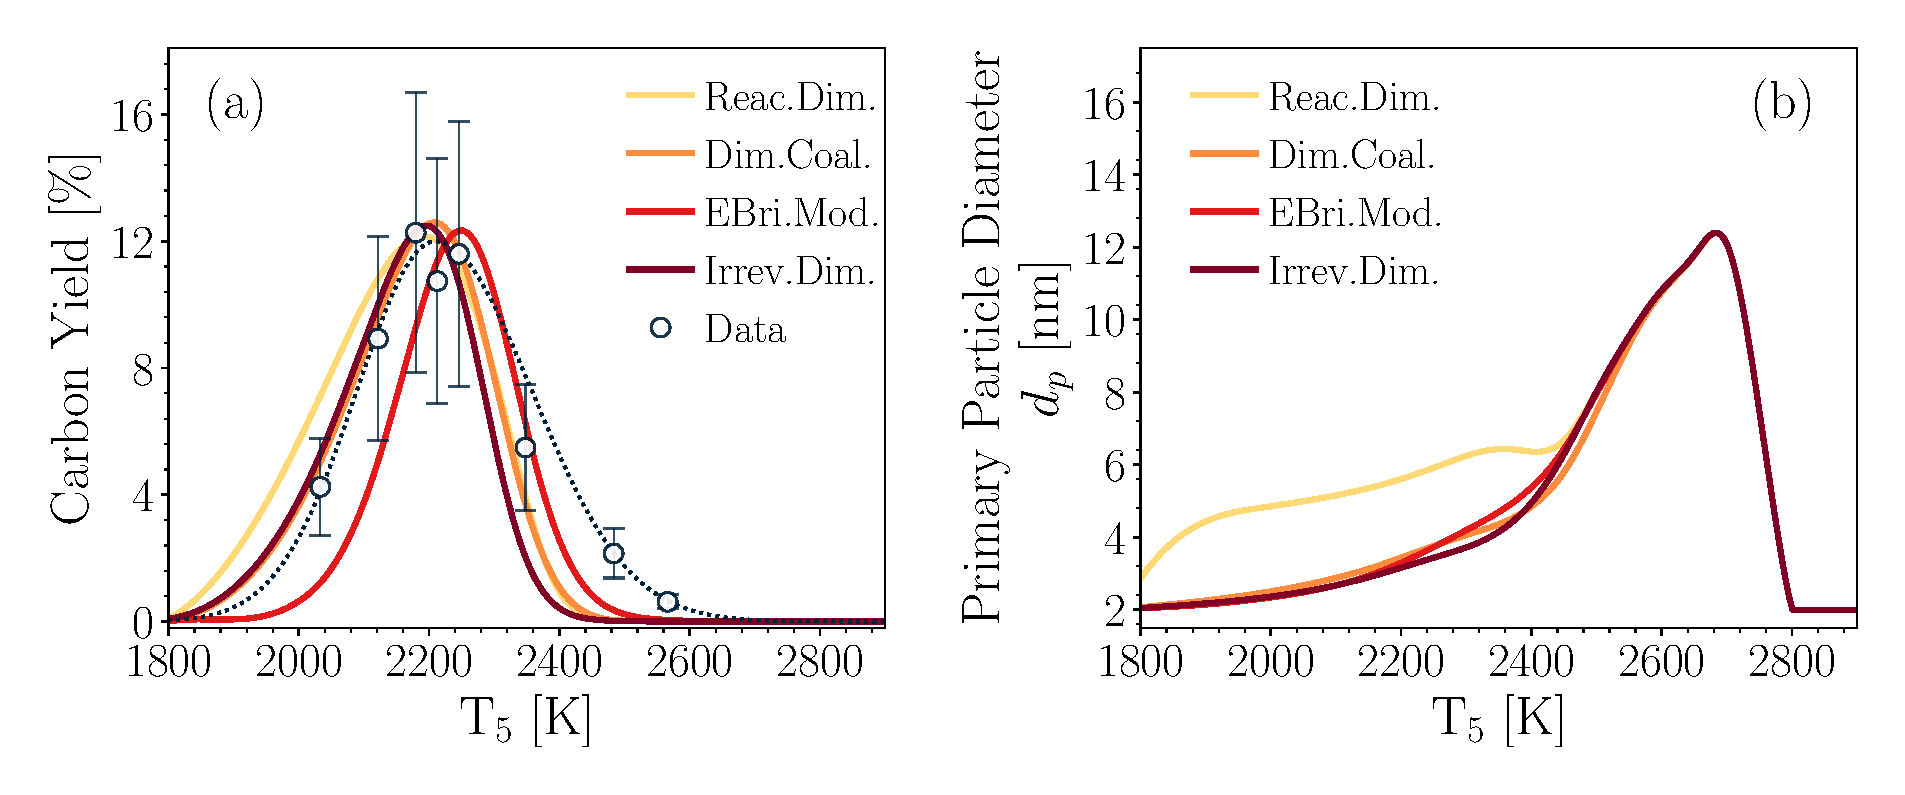
\includegraphics[width=0.8\textwidth]{Figures/Results/Shocktube/Agafonov2016_cpr/carbon_yield_d_p_5CH4.pdf}};
		\draw (-0.85, 0.42) node {\scriptsize{\cite{agafonov2016unified}}};
		%\draw (2.42, -0.23) node {\scriptsize{\cite{agafonov2016unified}}};
	\end{tikzpicture}
	\caption{The CY (a) and primary particle diameter, $d_p$, at $t=$1.5 ms obtained  using Caltech mechanism, SPBM and different inception models optimized using equal adjustment factors to minimize the prediction error with extinction measurements~\citep{agafonov2016unified}. The dashed line was added to show the trend in the measurements.}
	\label{fig:shockagof_yield_dp_cpr} 
\end{figure}


\begin{figure}[H]
	\centering
	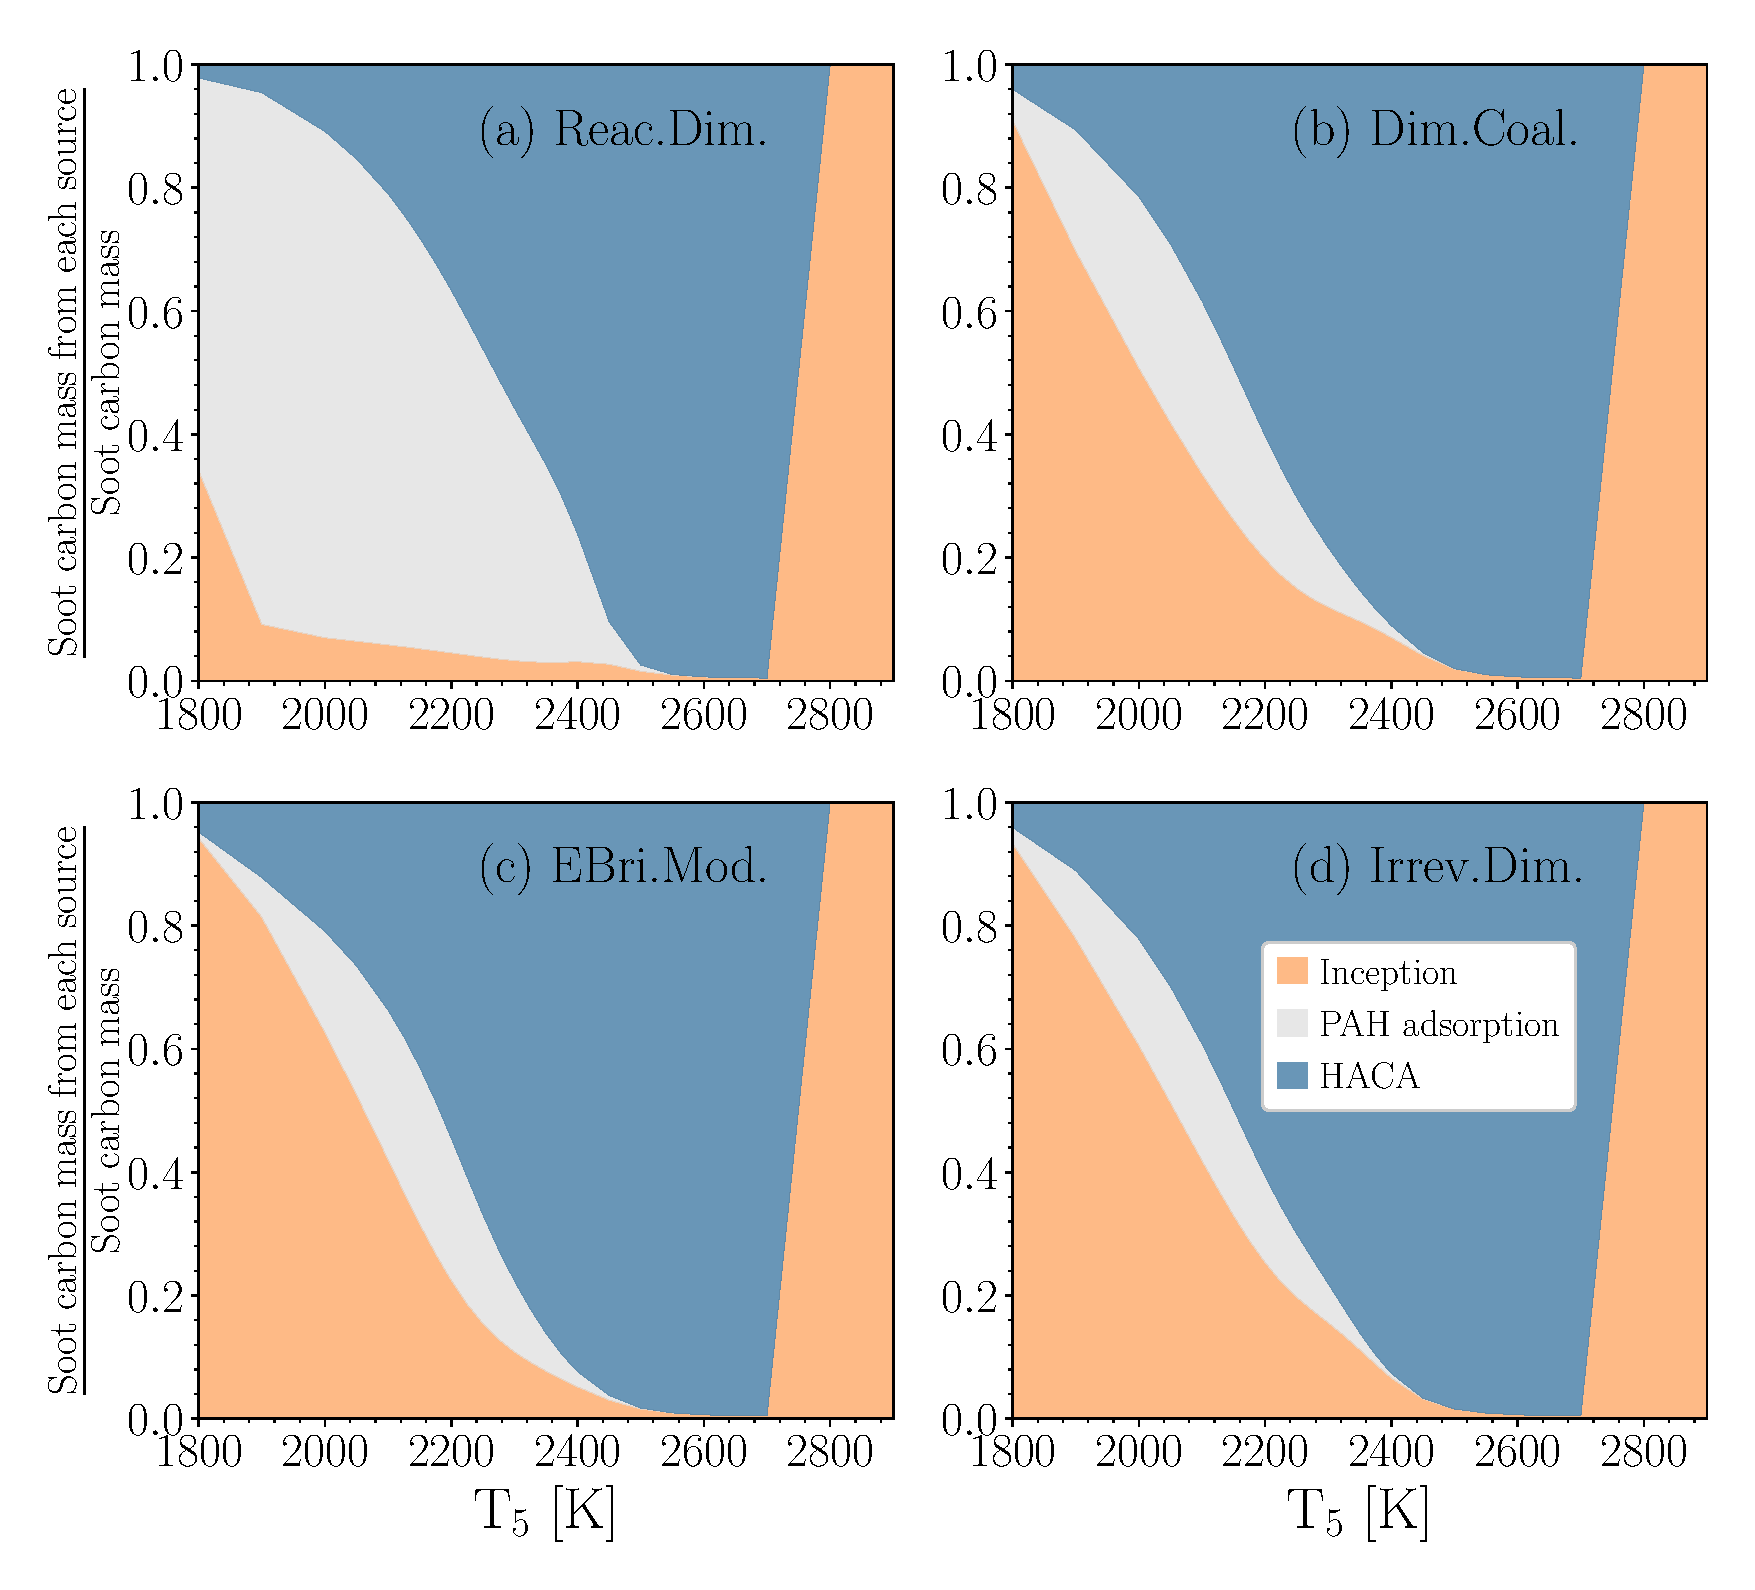
\includegraphics[width=0.8\textwidth]{Figures/Results/Shocktube/Agafonov2016_cpr/C_tot_distmap_5CH4.pdf}
	\caption{The soot carbon mass from inception, PAH adsorption and HACA normalized by total soot carbon mass at $t=1.5$ ms for 5\%$\mathrm{CH_4}$-Ar obtained using Caltech mechanism, SPBM and different inception models calibrated to minimize the prediction error with extinction measurements~\citep{agafonov2016unified}.}
	\label{fig:shockagof_carbon_map_cpr} 
\end{figure}


\begin{figure}[H]
	\centering
	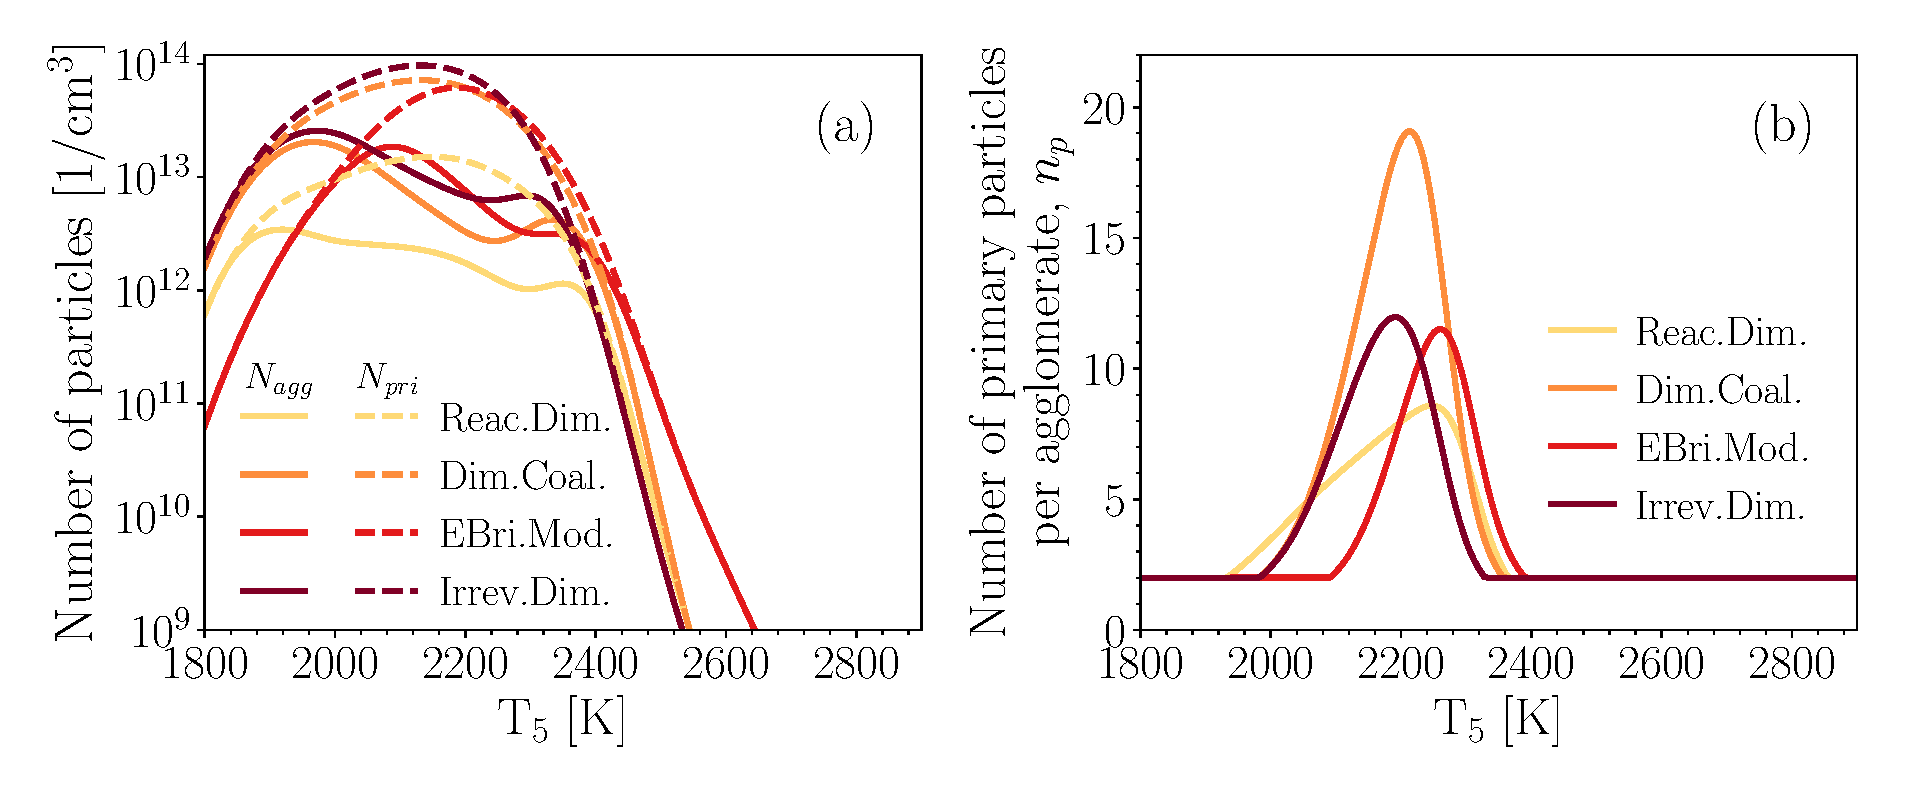
\includegraphics[width=0.8\textwidth]{Figures/Results/Shocktube/Agafonov2016_cpr/N_agg_n_p_5CH4.pdf}
	\caption{The temperature dependence of total number of agglomerates, $N_{agg}$ (a), number of primary particles per agglomerate, $n_p$ (b) at $t=$1.5 ms obtained using Caltech mechanism and different inception models optimized using equal adjustment factors to minimize the prediction with extinction measurements~\citep{agafonov2016unified}.}
	\label{fig:shockagof_Nagg_np_cpr} 
\end{figure}



Figure~\ref{fig:shockagof_yield_maxincads_cpr} shows that the optimized models with minimum $\eta_{inc}$ and $\eta_{ads}$ yields similar CY across inception models, except E-Bridge Modified model, which shifts slightly toward higher temperatures. The minimum adsorption case has a higher peak and narrower profile compared to the minimum inception case. As shown in Figure~\ref{fig:shockagof_dp_maxincads_cpr}, $d_p$ predicted in Min-Ads mode is smaller and less sensitive to the selection of inception model compared to Min-Inc mode. Two peaks can be seen in Min-Inc mode for all inception models: The first peak occurs due to high PAH adsorption rates at the temperature range close to the peak of CMF of soot precursors (Figure~\ref{fig:SPC_cmf_cpr}a); the second peak which occurs around $\mathrm{T_5}=$2700 K and $d_p=12$ nm, which is very similar to $d_p$ trends predicted using equal adjustment factors (Figure~\ref{fig:shockagof_yield_dp_cpr}b). Reactive Dimerization model has the largest variation at the peak from 2 to 19~nm between Min-Ads and Min-Inc modes. The existence of such a variation highlight the need for characterizing primary particle size in the experiment to reduce the uncertainty in the soot model and restrict the range of expected inception and surface growth rate required to accurately predict soot yield and morphology.

\begin{figure}[H]
	\centering
	\begin{tikzpicture}
			\draw (0, 0) node[inner sep=0] 	{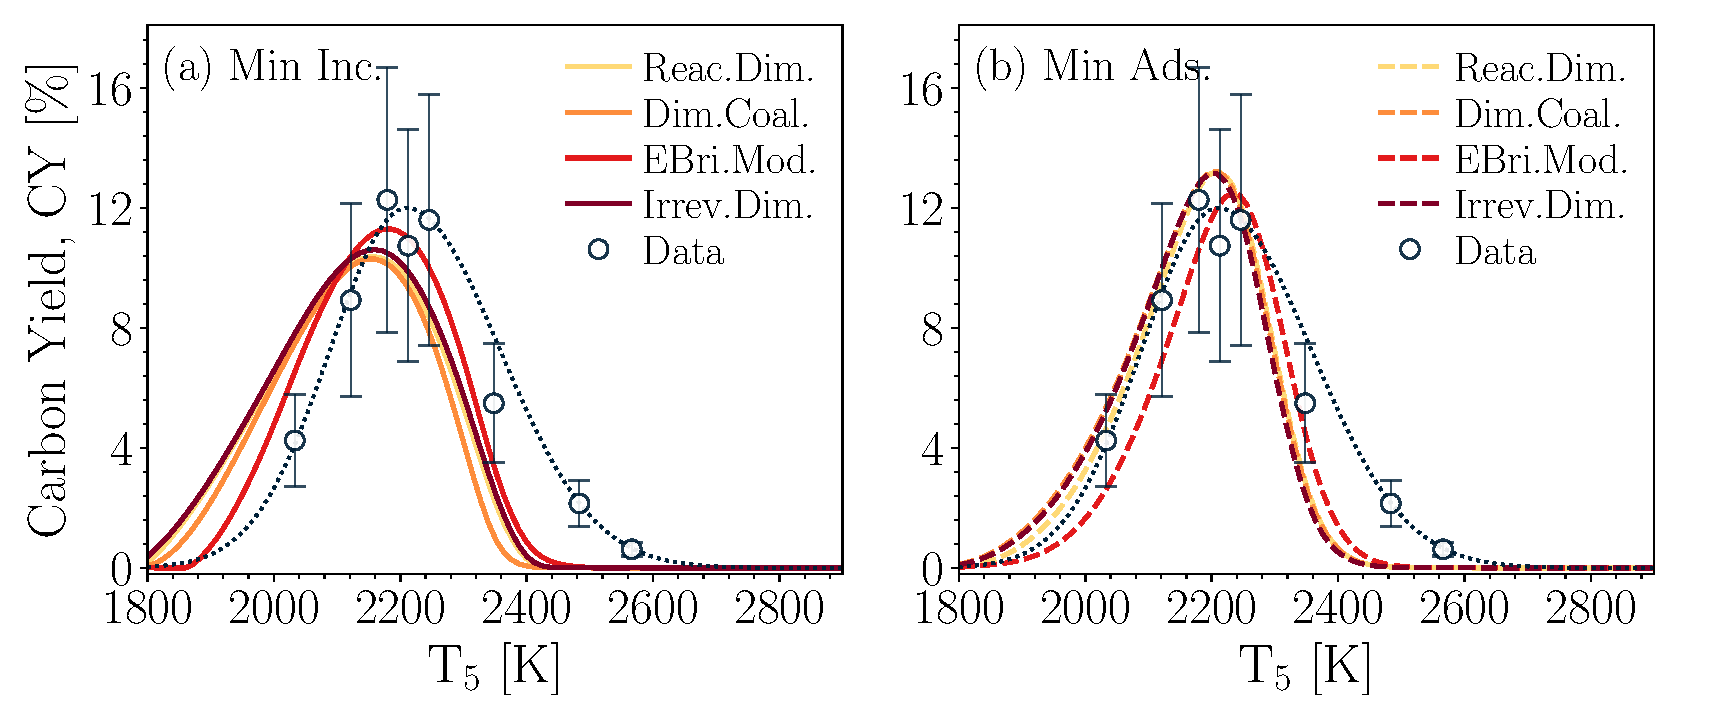
\includegraphics[width=0.8\textwidth]{Figures/Results/Shocktube/Agafonov2016_cpr/carbon_yield_maxincads_combined.pdf}};
			\draw (-0.48, 0.75) node {\scriptsize{\cite{agafonov2016unified}}};
			\draw (5.33, 0.75) node {\scriptsize{\cite{agafonov2016unified}}};
		\end{tikzpicture}
	\caption{The comparison of CY at $t=$1.5 ms when the minimum inception (a) and the minimum PAH adsorption (b) adjustment factors were applied to minimize the prediction error compared with the measurements~\citep{agafonov2016unified} for 5\%~$\mathrm{CH_4}$-Ar obtained using Caltech mechanism, SPBM and different inception models.}
	\label{fig:shockagof_yield_maxincads_cpr} 
\end{figure}

%\begin{figure}[H]
%	\centering
%	\begin{tikzpicture}
%		\draw (0, 0) node[inner sep=0] 	{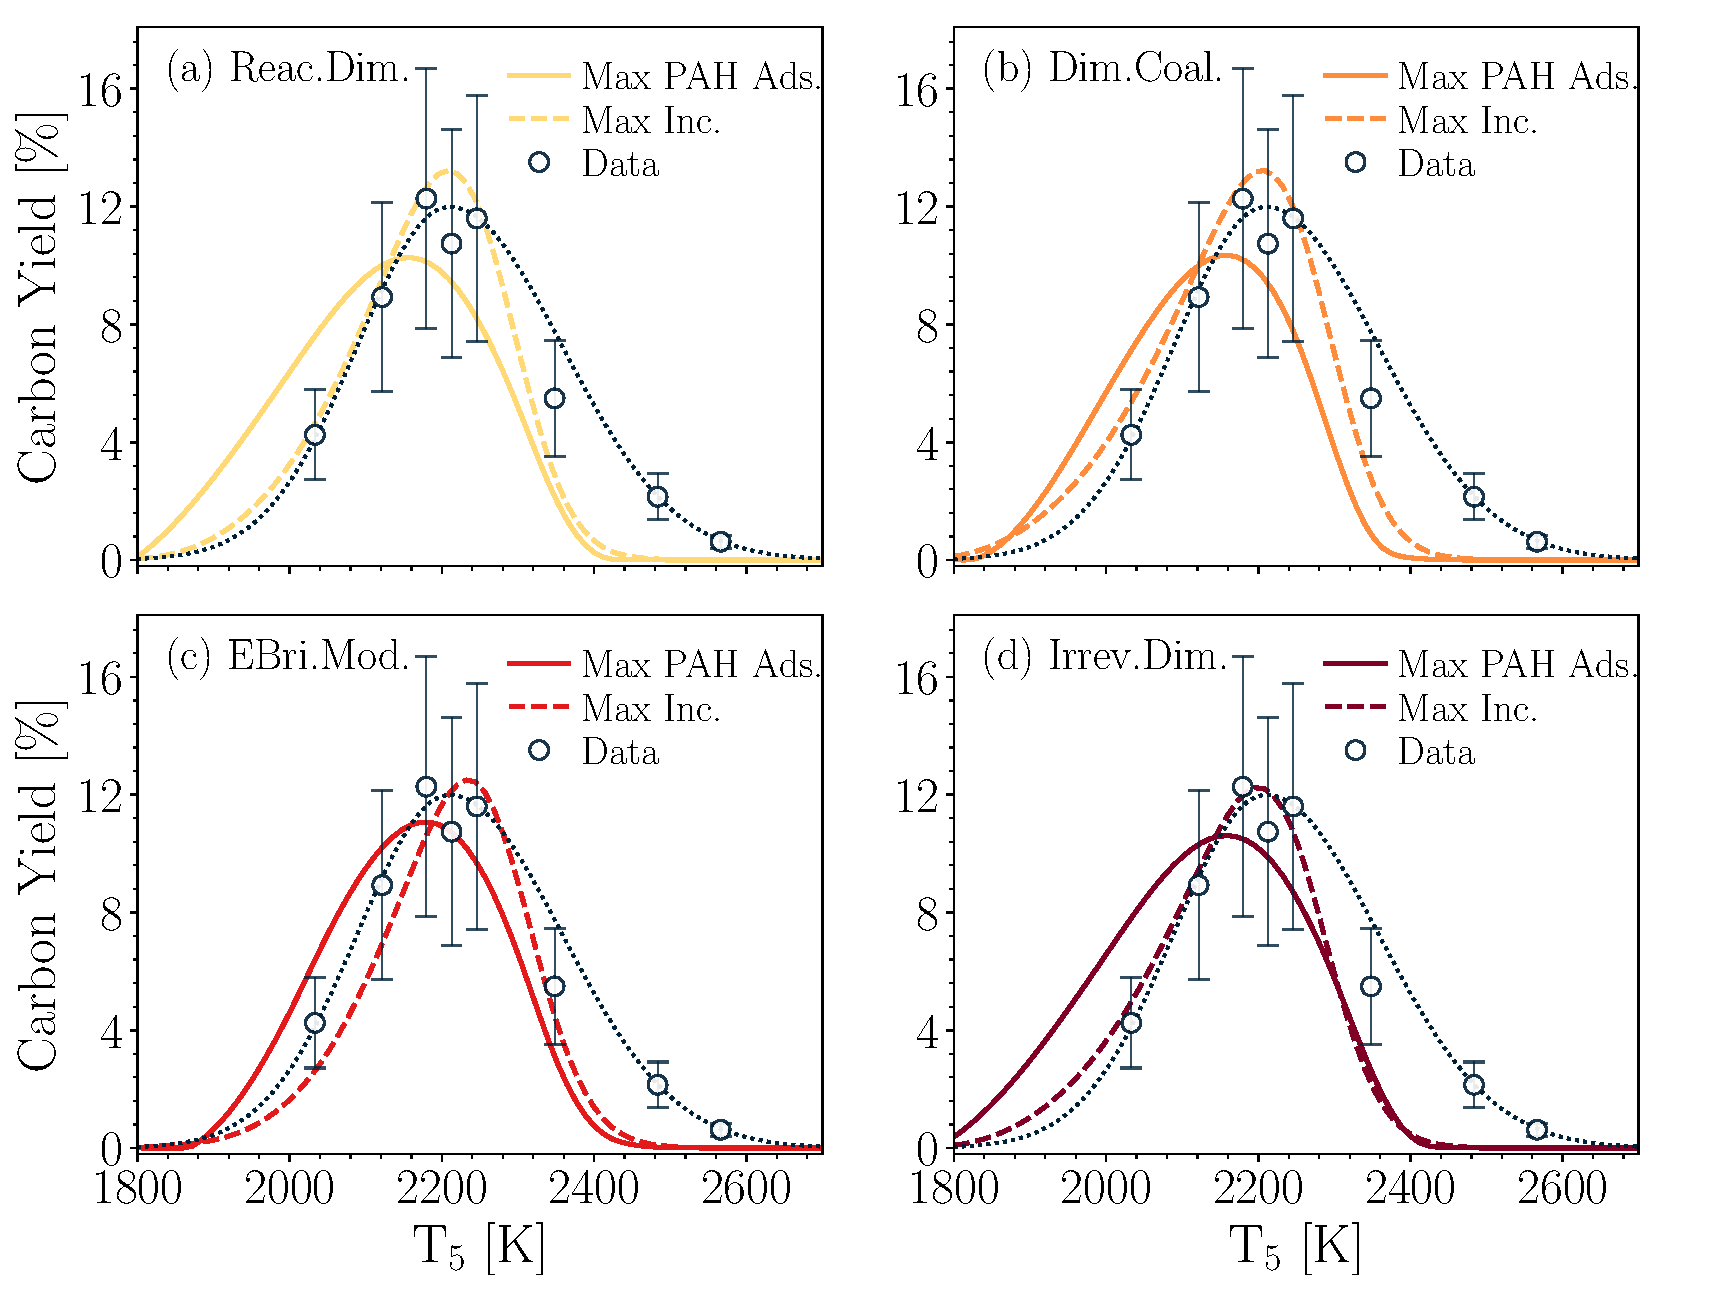
\includegraphics[width=0.8\textwidth]{Figures/Results/Shocktube/Agafonov2016_cpr/carbon_yield_maxincads.pdf}};
%		\draw (-0.48, -0.8) node {\scriptsize{\cite{agafonov2016unified}}};
%		\draw (5.33, -0.8) node {\scriptsize{\cite{agafonov2016unified}}};
%		\draw (-0.48, 3.36) node {\scriptsize{\cite{agafonov2016unified}}};
%		\draw (5.33, 3.36) node {\scriptsize{\cite{agafonov2016unified}}};
%	\end{tikzpicture}
%	\caption{The comparison of soot carbon yield at t=1.5 ms when maximum inception (dashed line) and PAH adsorption (solid line) were applied to minimized the prediction error compared to measurements~\citep{agafonov2016unified} for 5\% (a) and 10\%~$\mathrm{CH_4}$ (b) in Ar obtained using Caltech mechanism and different inception models.}
%	\label{fig:shockagof_yield_maxincads_cpr} 
%\end{figure}

\begin{figure}[H]
	\centering
	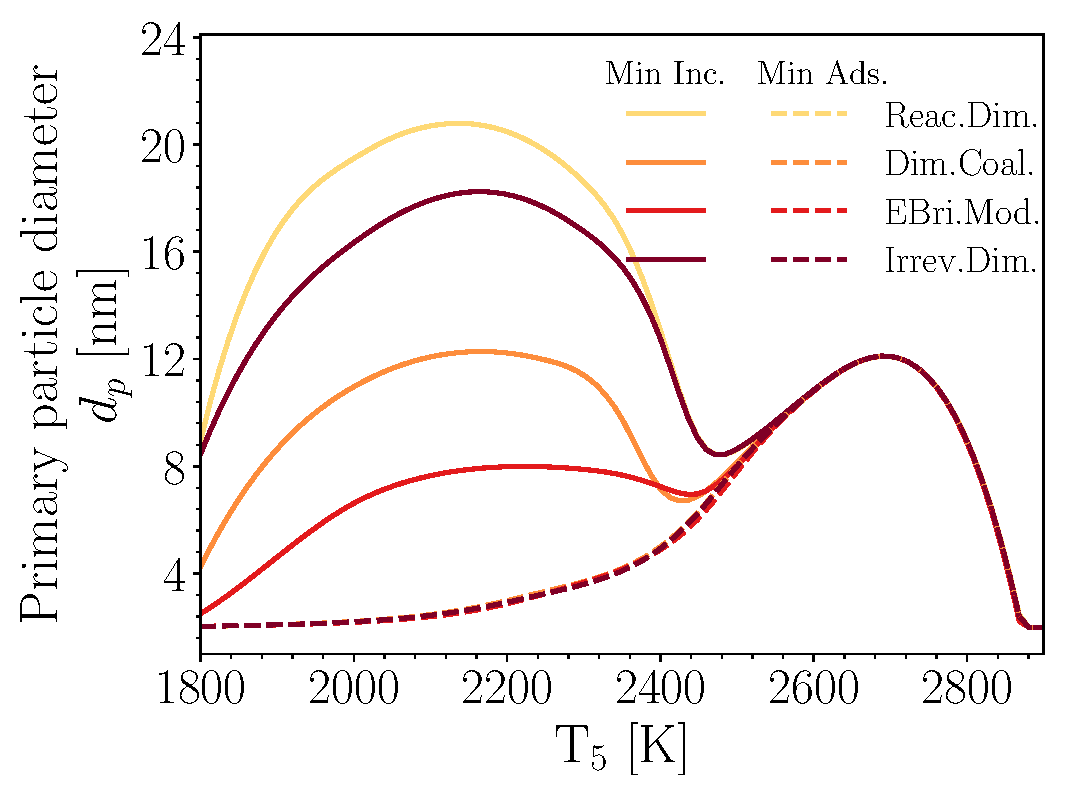
\includegraphics[width=0.5\textwidth]{Figures/Results/Shocktube/Agafonov2016_cpr/d_p_maxincads_combined.pdf}
	\caption{The comparison of mean primary particle, $d_p$, at $t=$1.5 ms when the minimum inception (solid lines) and adsorption (dashed lines) were applied to minimized the prediction error compared to measurements~\citep{agafonov2016unified} for 5\%$\mathrm{CH_4}$-Ar obtained using Caltech mechanism, SPBM and different inception models.}
	\label{fig:shockagof_dp_maxincads_cpr} 
\end{figure}

%\begin{figure}[H]
%	\centering
%	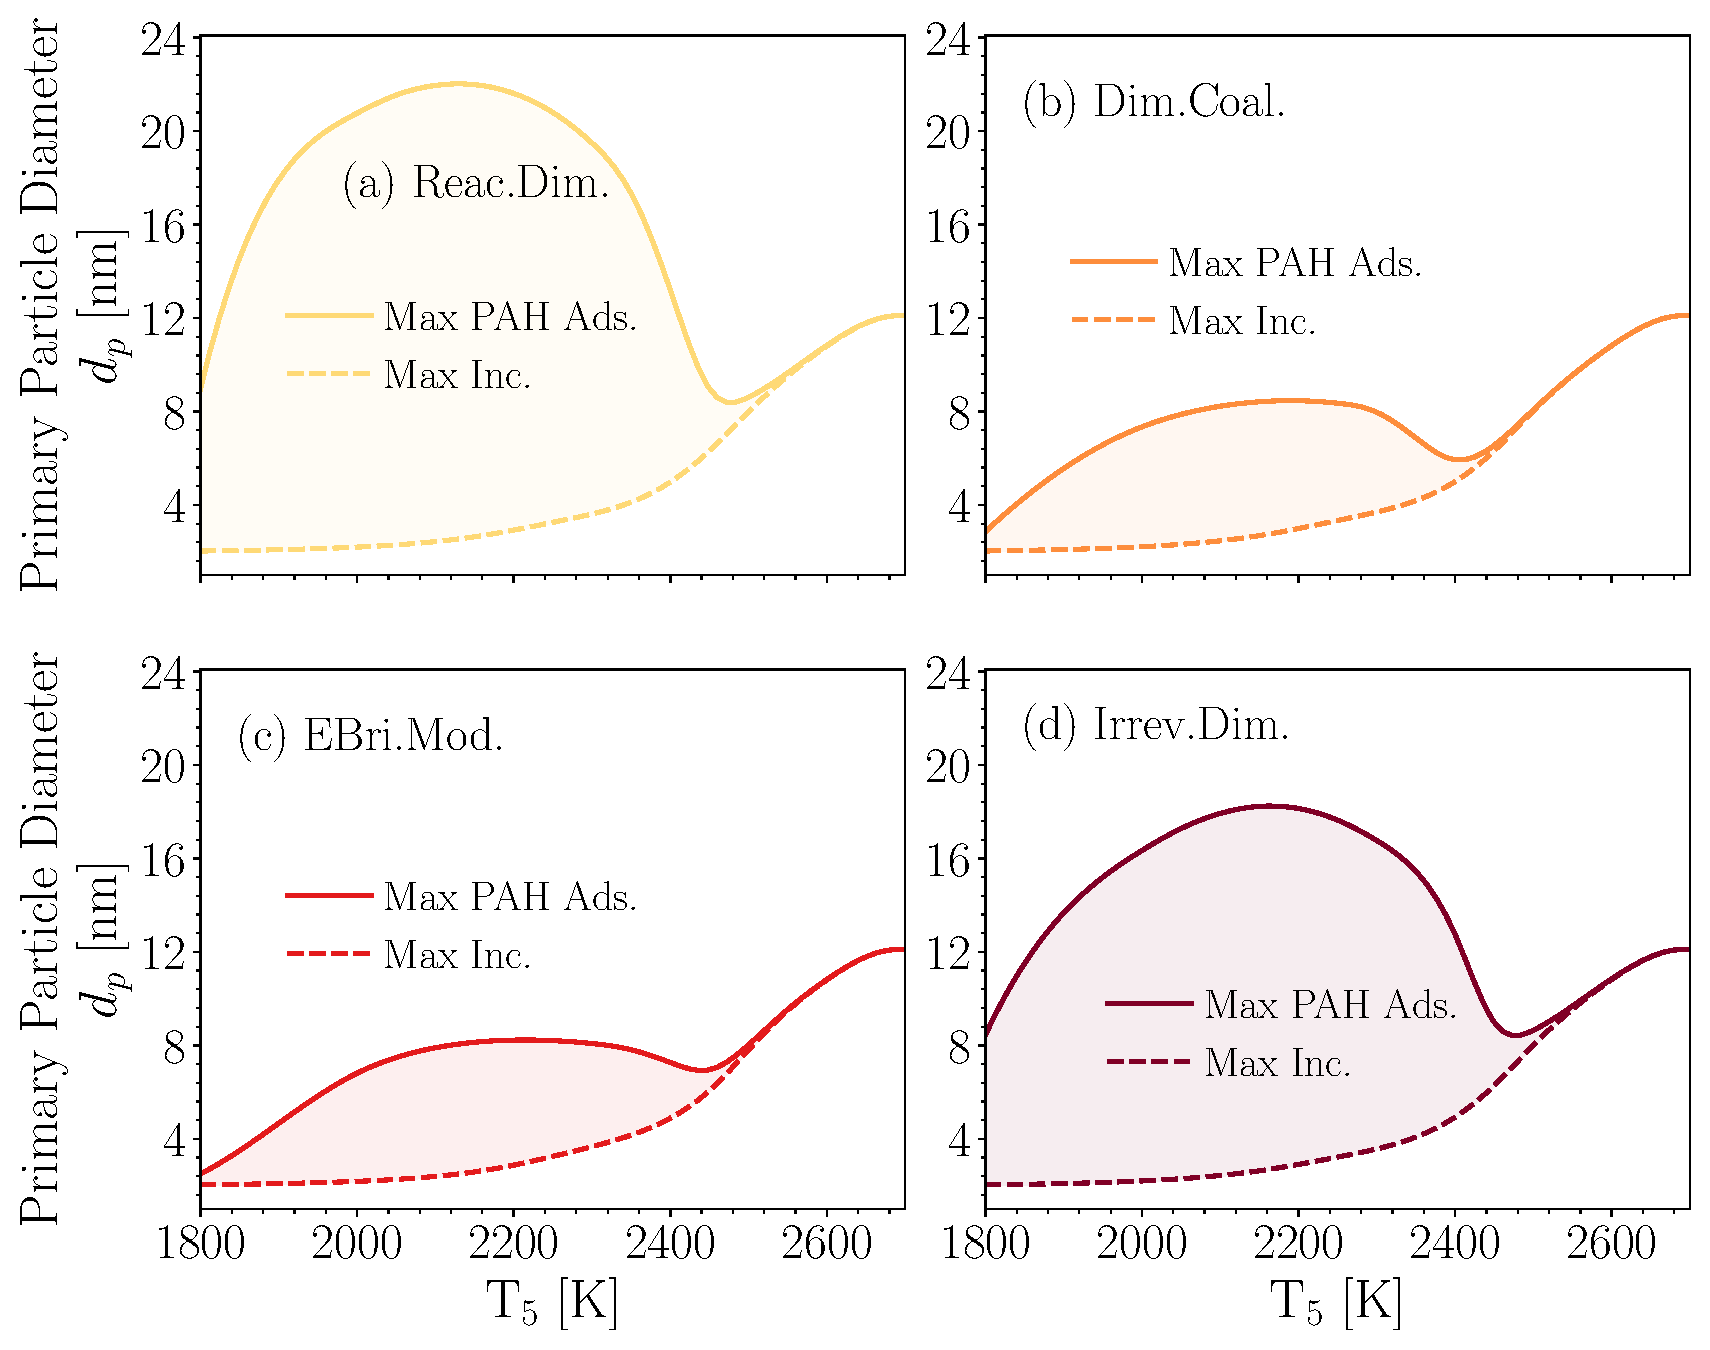
\includegraphics[width=0.8\textwidth]{Figures/Results/Shocktube/Agafonov2016_cpr/d_p_maxincads.pdf}
%	\caption{The comparison of mean primary particle, $d_p$ at t=1.5 ms when maximum inception and PAH adsorption were applied to minimized the prediction  error compared to measurements~\citep{agafonov2016unified} for 5\% (a) and 10\%~$\mathrm{CH_4}$ (b) in Ar obtained using Caltech mechanism and different inception models.}
%	\label{fig:shockagof_dp_maxincads_cpr} 
%\end{figure}

%\subsection{Methane pyrolysis in shock-tube using constant volume reactor}

%The pyrolysis of 5\% and 10\% $\mathrm{CH_4}$-Ar was investigated using a constant volume reactor model (CVR) for the post-shock temperature, $T_5$ range of 1800-3000 K, and pressure, $P_5$ range of 4.7-7.1 bar. $P_5$ was assumed to linearly increase with $T_5$ across the simulation cases. Caltech mechanism was used and the inception models were calibrated in order to match carbon yield at t=1.5 ms with the measurement~\citep{agafonov2016unified} using a dual-beam absorption–emission technique. \citet{agafonov2016unified} reported yield$\times$E(m) at $\mathrm{\lambda}$=632~nm, and yield data was retrieved using E(m)=0.37 suggested therein. 


%\begin{figure}[H]
%	\centering
%	\begin{subfigure}[t]{0.4\textwidth}
%		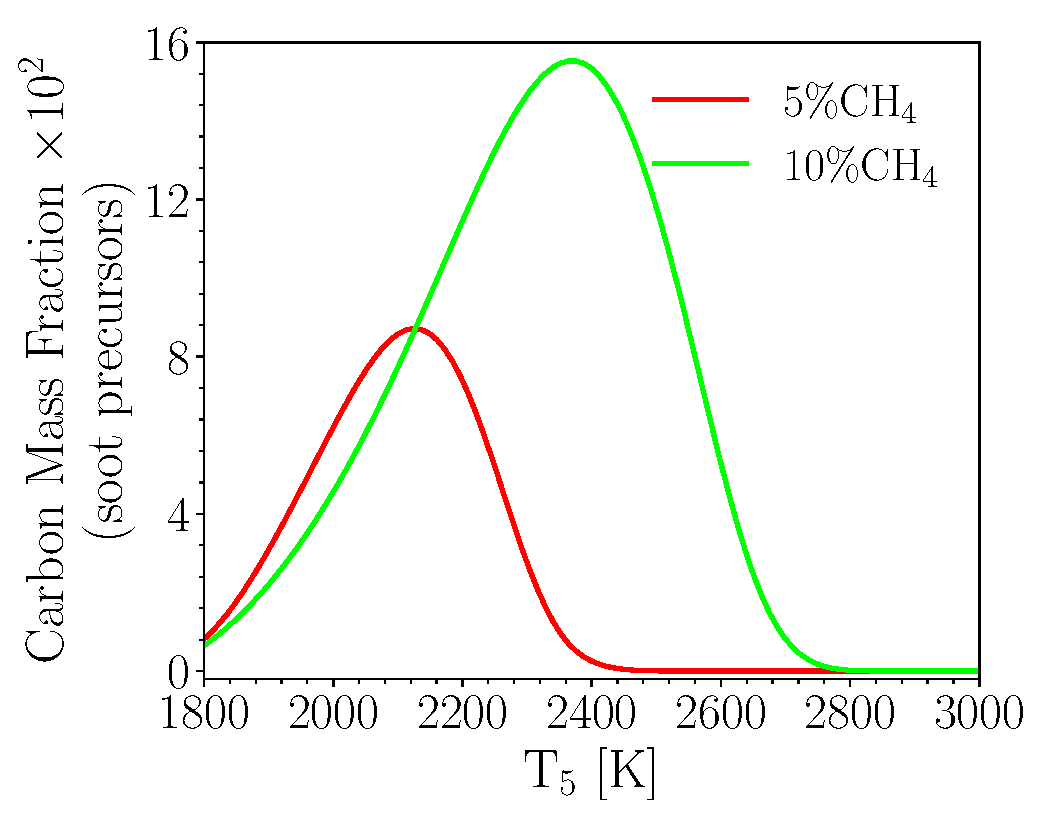
\includegraphics[width=1\textwidth]{Figures/Results/Shocktube/Agafonov2016_cvr/SPC_cmf.pdf}
%	\end{subfigure}
%	\begin{subfigure}[t]{0.4\textwidth}
%		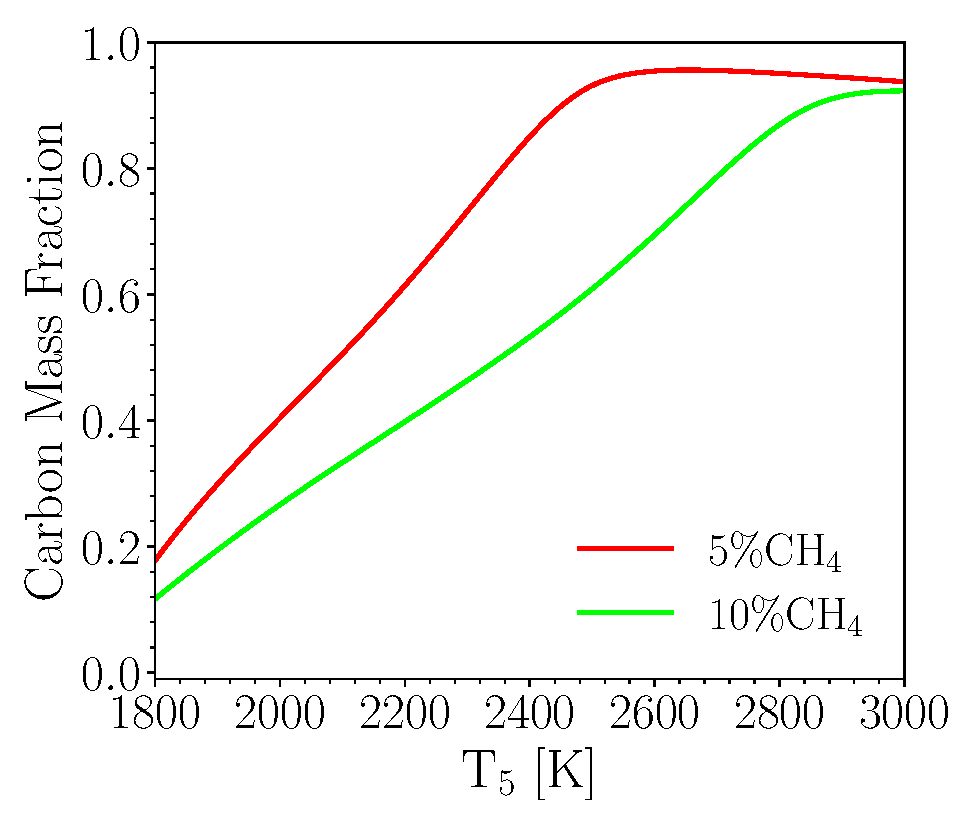
\includegraphics[width=1\textwidth]{Figures/Results/Shocktube/Agafonov2016_cvr/C2H2_cmf.pdf}
%	\end{subfigure}
%	\caption{The bell-shape temperature profile of carbon mass fraction of soot precursors (A2 and larger) combined (a) and $\mathrm{C_2H_2}$ (b) at t=1.5 ms during pyrolysis of 5\% (red line) and 10\%~$\mathrm{CH_4}$-Ar (green line) obtained using Caltech mechanism without considering soot}
%	\label{fig:SPC_cmf_cvr} 
%\end{figure}
%
%
%
%
%\begin{figure}[H]
%	\centering
%	\begin{tikzpicture}
%		\draw (0, 0) node[inner sep=0] 	{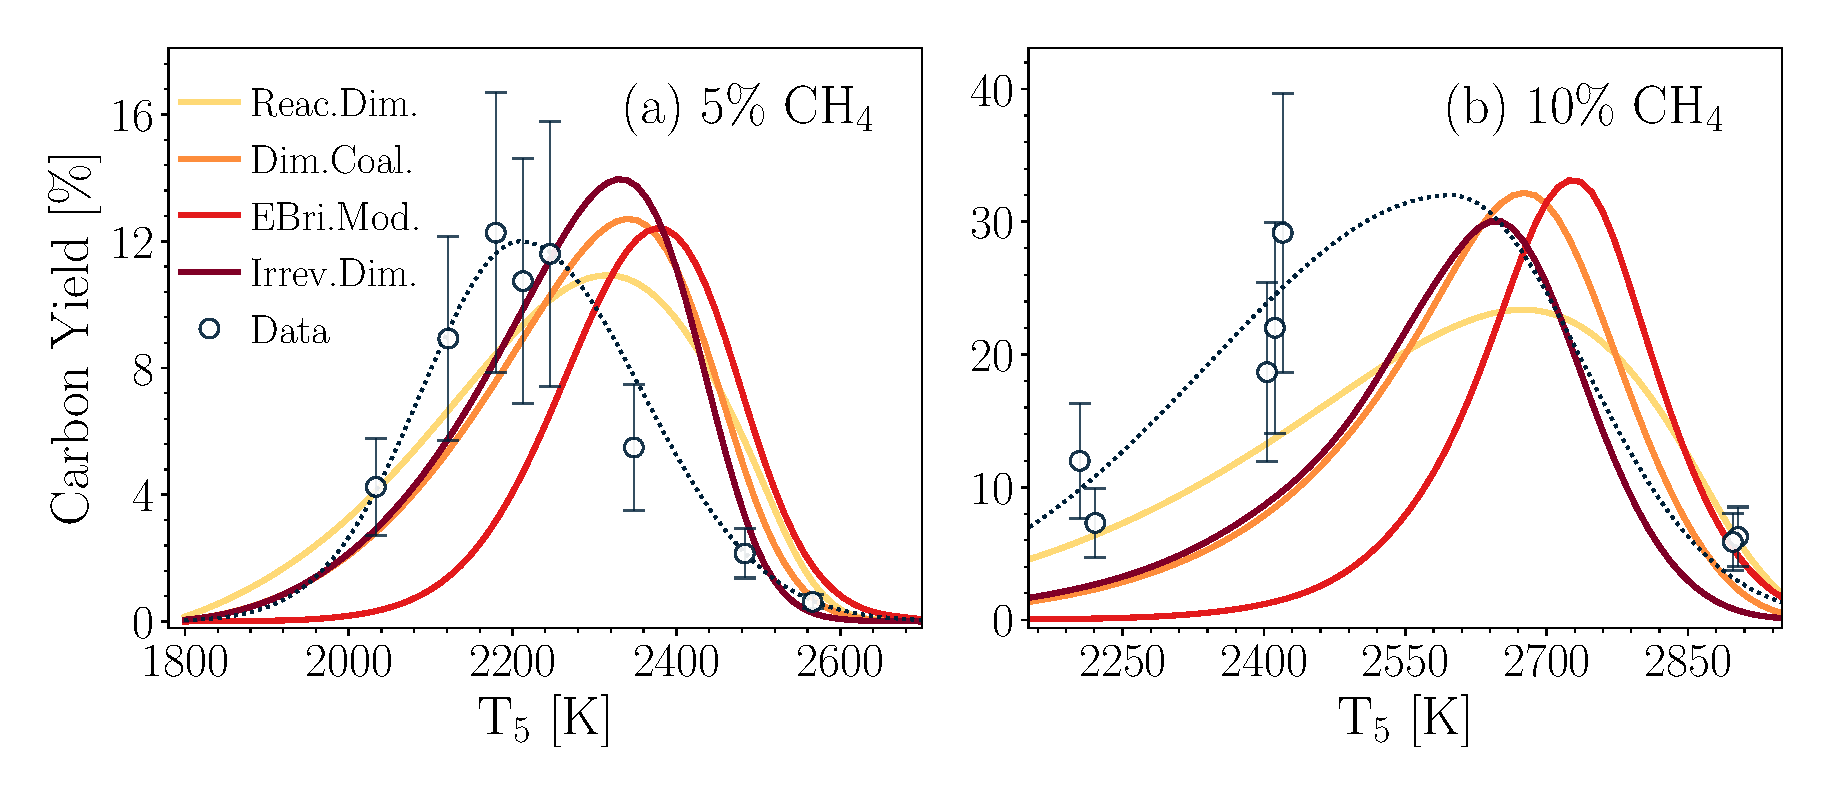
\includegraphics[width=0.8\textwidth]{Figures/Results/Shocktube/Agafonov2016_cvr/carbon_yield.pdf}};
%		\draw (-3.6, 0.42) node {\scriptsize{\cite{agafonov2016unified}}};
%		%\draw (2.42, -0.23) node {\scriptsize{\cite{agafonov2016unified}}};
%	\end{tikzpicture}
%	\caption{The bell-shape temperature profile of soot carbon yield at t=1.5 ms for 5\% (a) and 10\%~$\mathrm{CH_4}$ (b) in Ar obtained using Caltech mechanism and different inception models calibrated to minimize the prediction with extinction measurements~\citep{agafonov2016unified}.}
%	\label{fig:shockagof_yield_cvr} 
%\end{figure}
%
%Figure~\ref{fig:shockagof_yield} shows soot carbon yield predicted using Caltech mechanism where inception flux and PAH adsorption rate were adjusted using a scaling factor (equal for the both) to minimize the prediction error compared to the data from extinction measurements~\citep{agafonov2016unified}. A skew exponential curve fit (represented by the black dotted line) was applied to illustrate the trend in soot yield and identify the temperature at which the yield likely reaches its maximum. The predicted temperature of peak yield is larger than peak of curve-fit in both $\mathrm{CH_4}$ concentrations by 100-200 K depending on the inception model. This difference is due the contribution of  HACA to surface growth that depends on $\mathrm{C_2H_2}$ concentration which increases with temperature.
%
%\begin{figure}[H]
%	\centering
%	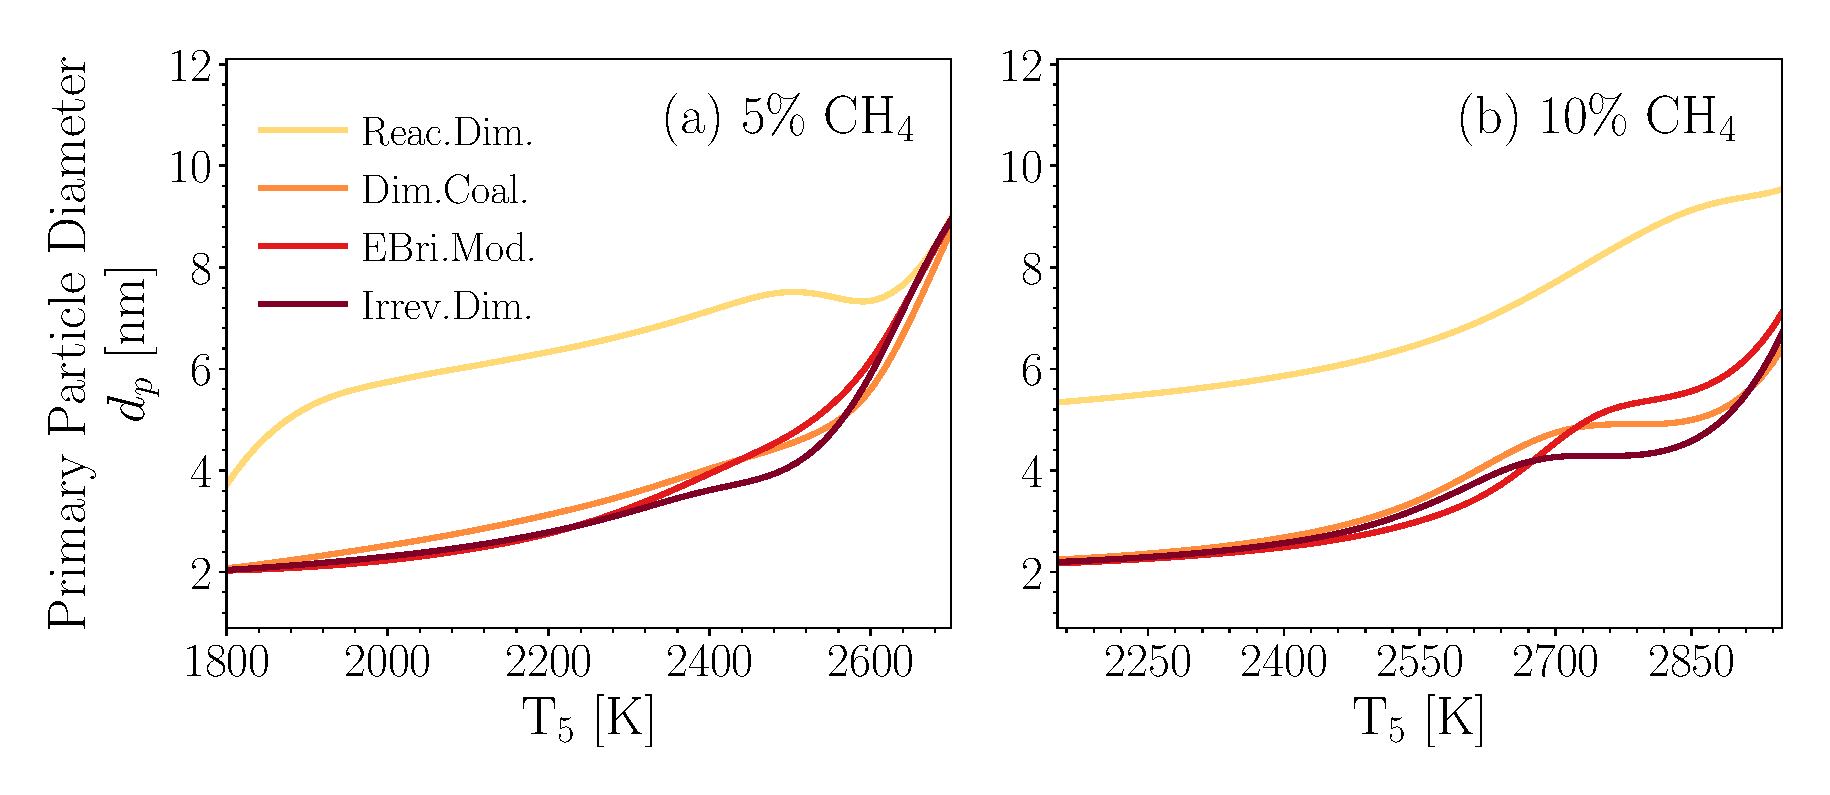
\includegraphics[width=0.8\textwidth]{Figures/Results/Shocktube/Agafonov2016_cvr/d_p.pdf}
%	\caption{The temperature dependence of mean primary particle diameter, $d_p$ at t=1.5 ms for 5\% (a) and 10\%~$\mathrm{CH_4}$ (b) in Ar obtained using Caltech mechanism and different inception models calibrated to minimize the prediction with extinction measurements~\citep{agafonov2016unified}.}
%	\label{fig:shockagof_dp_cvr} 
%\end{figure}
%
%Figure\ref{fig:shockagof_dp} shows that $d_p$ increases with temperature up to 10 nm. For 5\% $\mathrm{CH_4}$, $d_p$ reaches the peak around 2800 K and drops quickly to 2 nm which is the minimum allowed diameter in the model. Reactive Dimerization results in overall larger primary particle diameters, but the behavior of the rest of inception models are similar.
%
%\begin{figure}[H]
%	\centering
%	\begin{tikzpicture}
%		\draw (0, 0) node[inner sep=0] 	{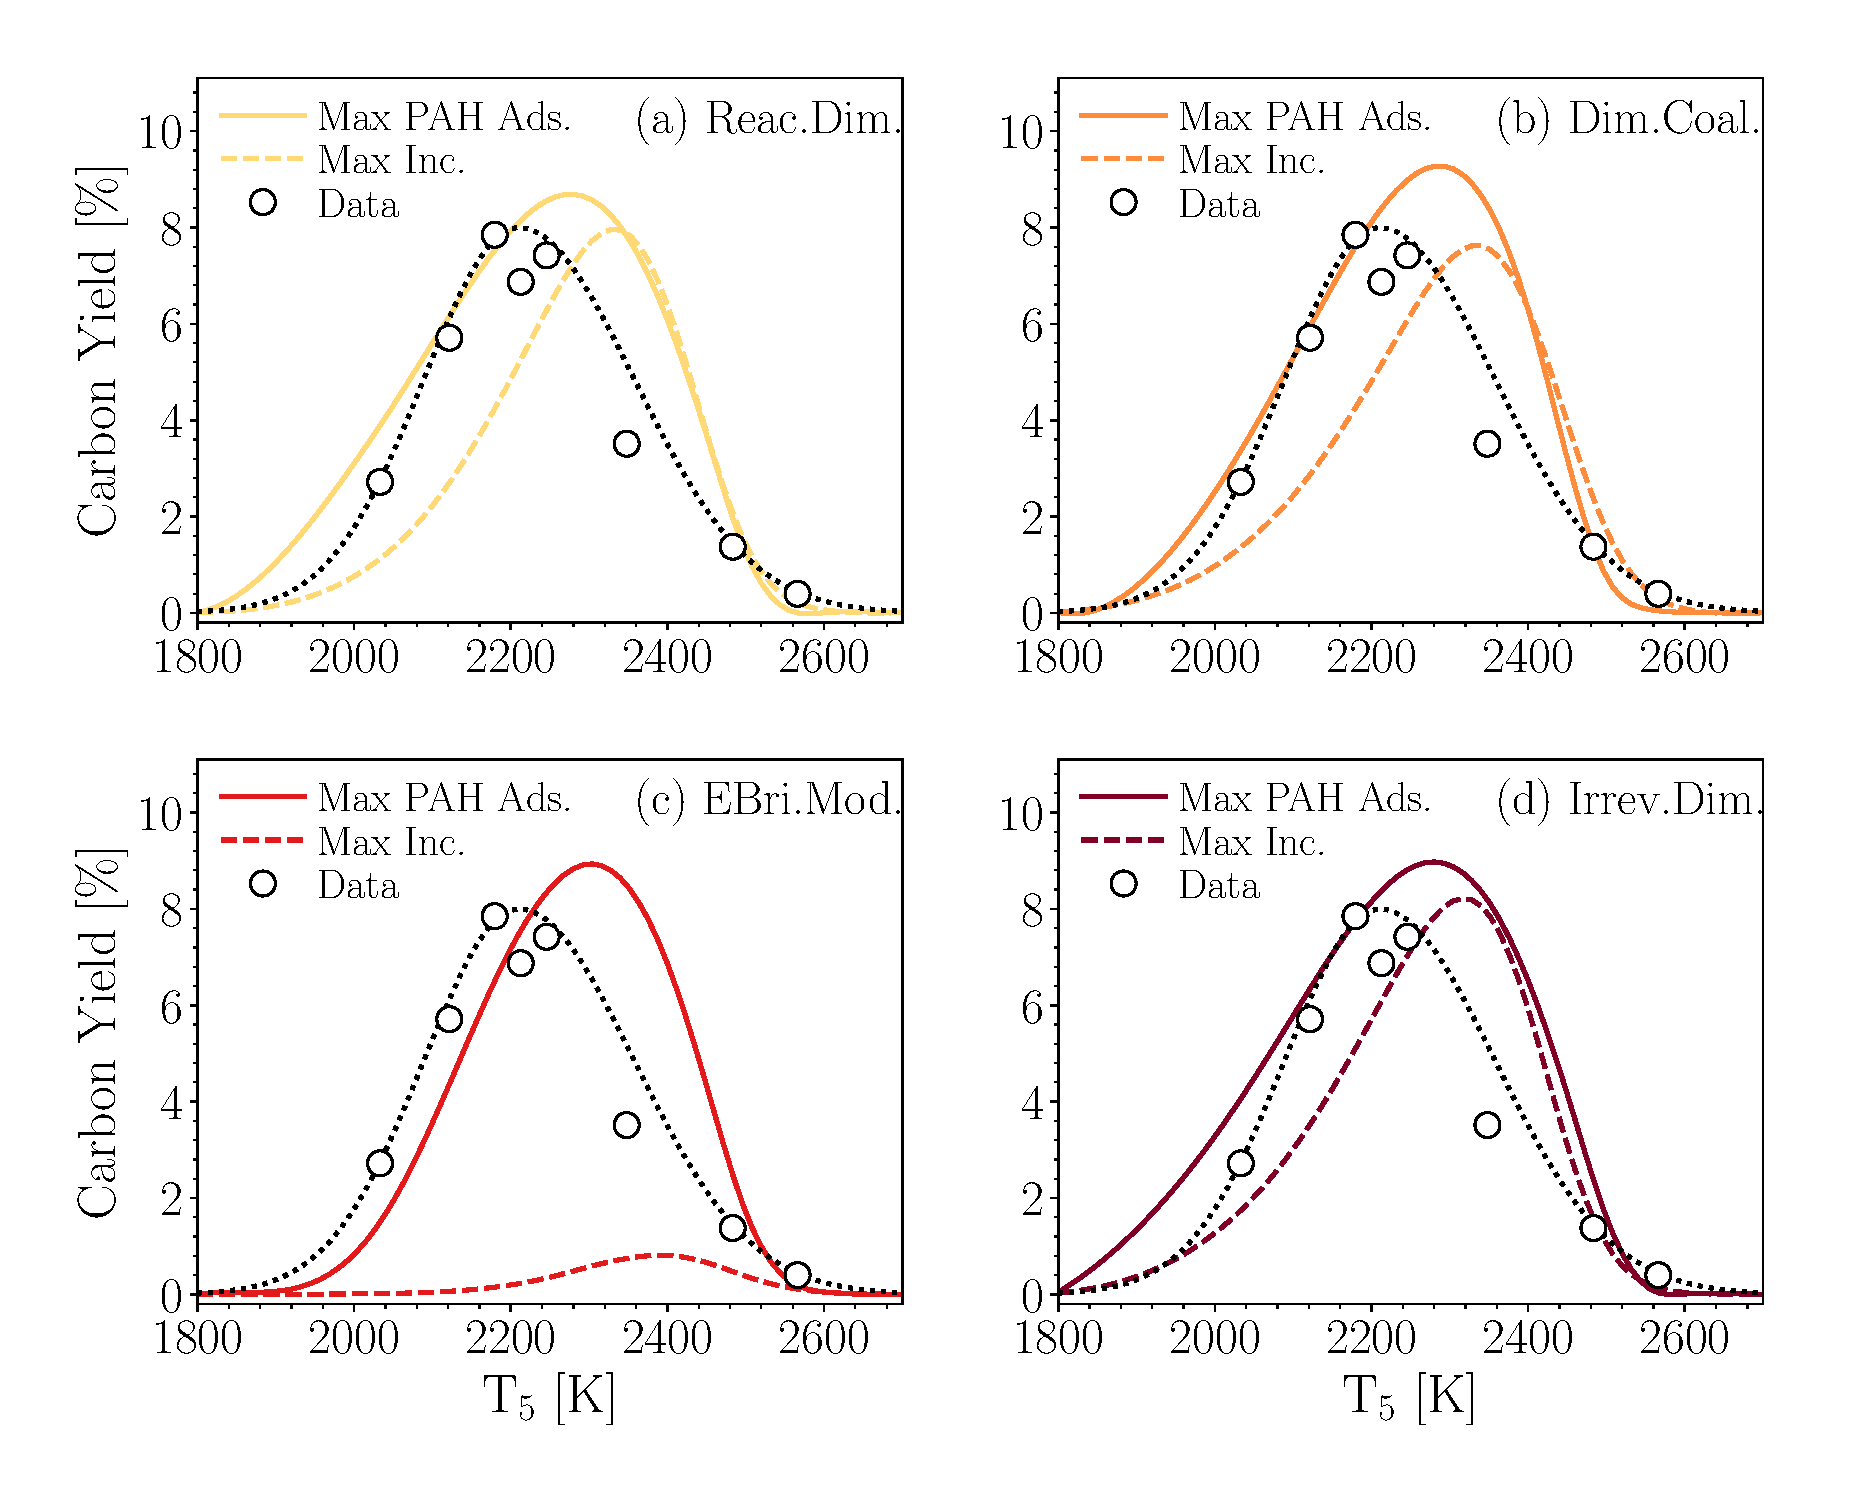
\includegraphics[width=0.8\textwidth]{Figures/Results/Shocktube/Agafonov2016_cvr/carbon_yield_maxincads.pdf}};
%		\draw (-3.18, -0.9) node {\scriptsize{\cite{agafonov2016unified}}};
%		\draw (2.46, -0.9) node {\scriptsize{\cite{agafonov2016unified}}};
%		\draw (-3.18, 3.55) node {\scriptsize{\cite{agafonov2016unified}}};
%		\draw (2.46, 3.55) node {\scriptsize{\cite{agafonov2016unified}}};
%	\end{tikzpicture}
%	\caption{The comparison of soot carbon yield at t=1.5 ms when maximum inception and PAH adsorption were applied to minimized the prediction  error compared to measurements~\citep{agafonov2016unified} for 5\% (a) and 10\%~$\mathrm{CH_4}$ (b) in Ar obtained using Caltech mechanism and different inception models.}
%	\label{fig:shockagof_yield_maxincads_cvr} 
%\end{figure}
%
%\begin{figure}[H]
%	\centering
%	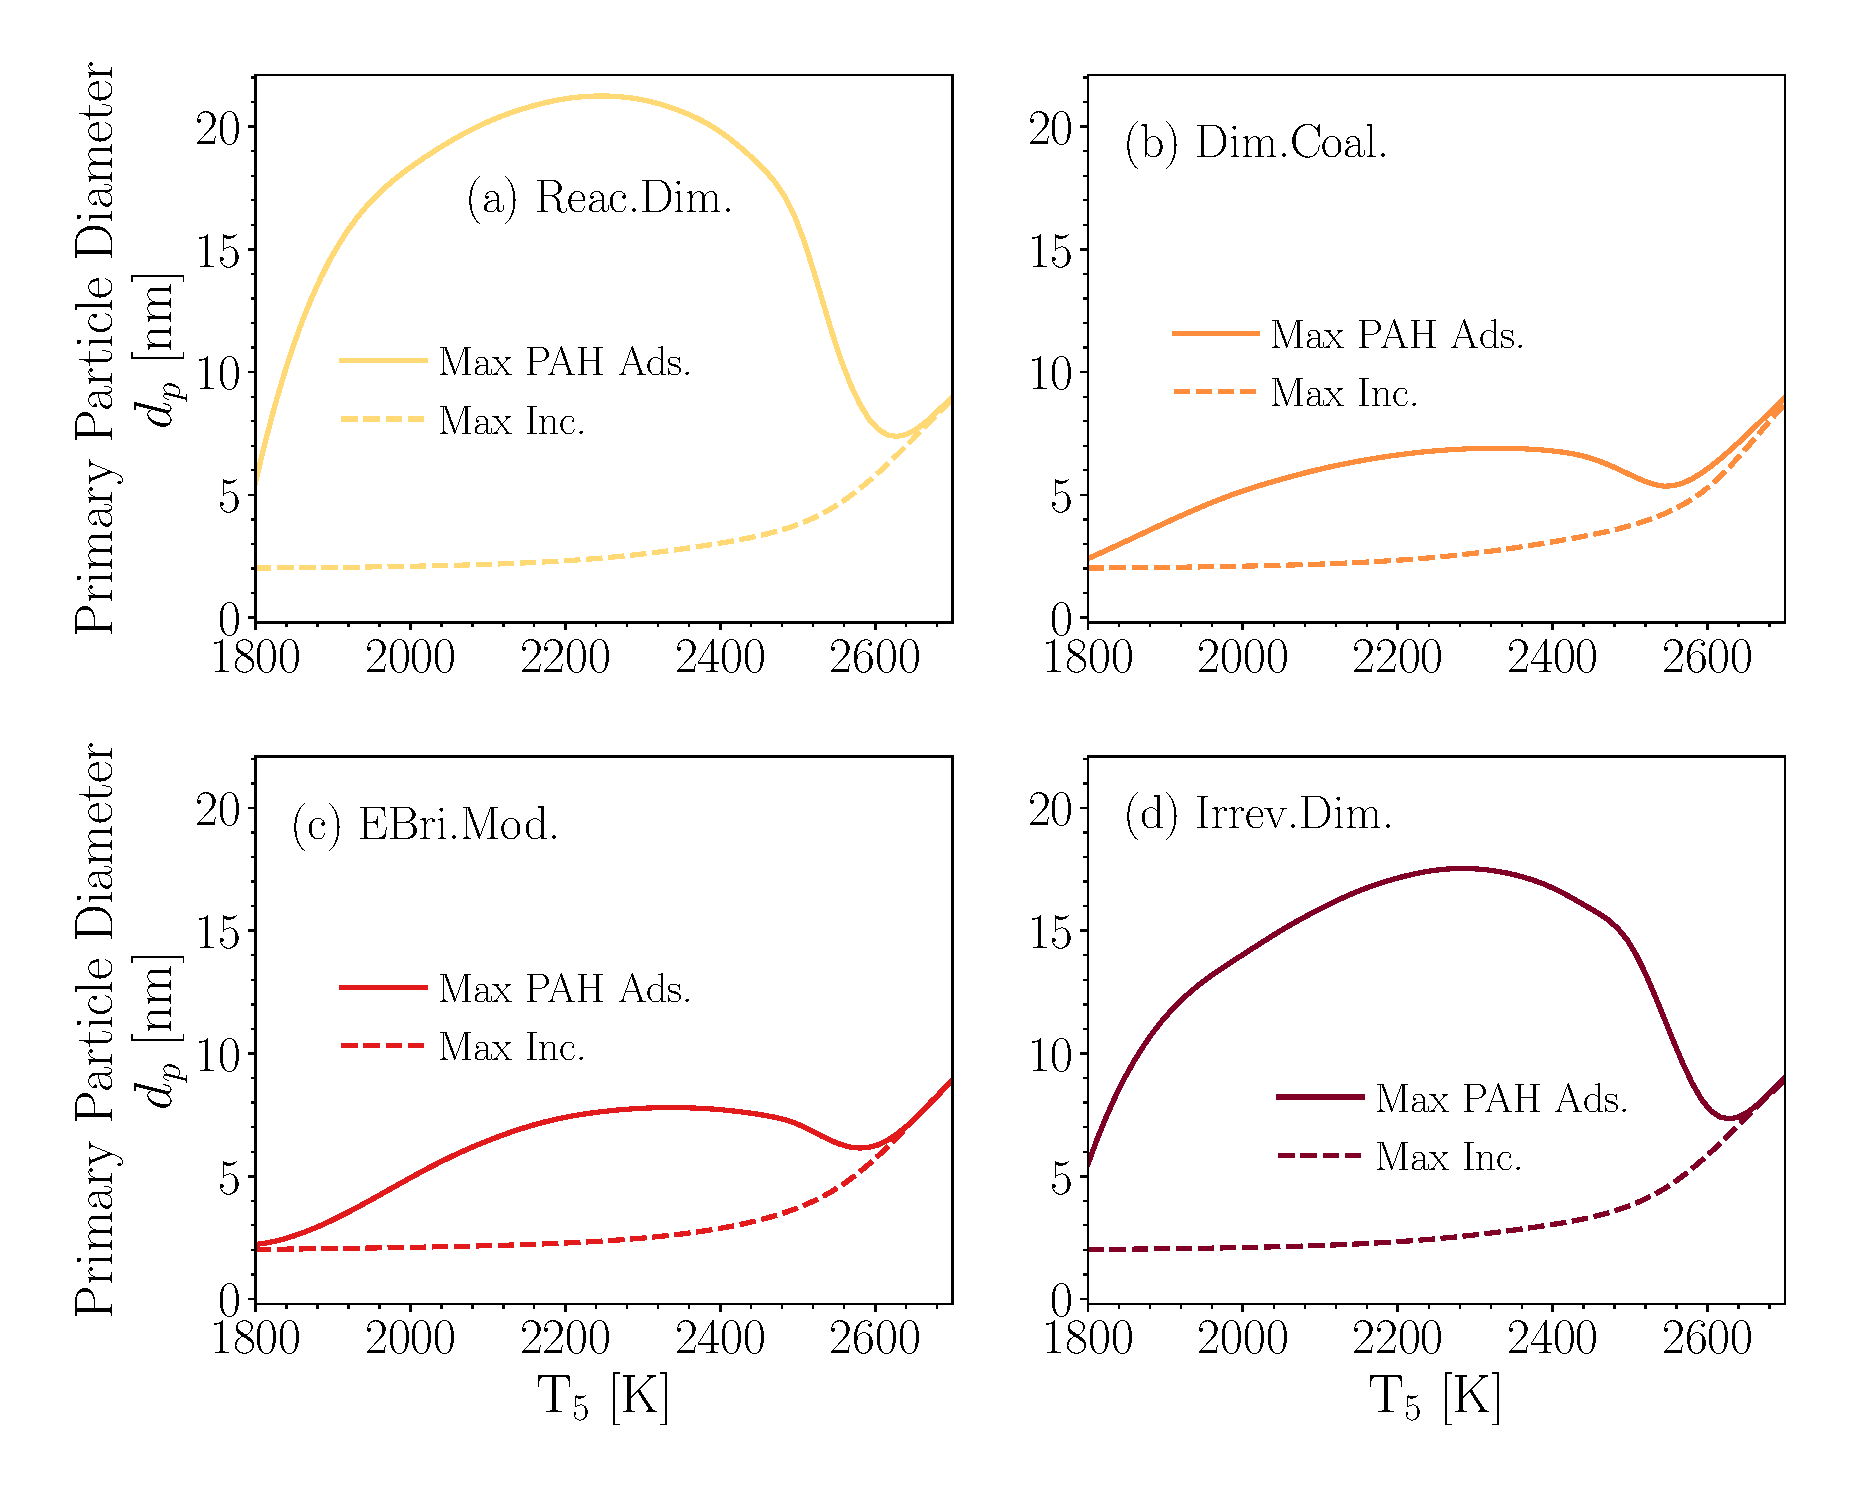
\includegraphics[width=0.8\textwidth]{Figures/Results/Shocktube/Agafonov2016_cvr/d_p_maxincads.pdf}
%	\caption{The comparison of mean primary particle, $d_p$ at t=1.5 ms when maximum inception and PAH adsorption were applied to minimized the prediction  error compared to measurements~\citep{agafonov2016unified} for 5\% (a) and 10\%~$\mathrm{CH_4}$ (b) in Ar obtained using Caltech mechanism and different inception models.}
%	\label{fig:shockagof_dp_maxincads_cvr} 
%\end{figure}